% Name: Request lifecycle
% Description: An HTTP request through a web framework: middleware, the router, a controller that asks the model for data, and the view that renders the response.
% Tags: request lifecycle, MVC, middleware, web framework

\usetikzlibrary{arrows.meta, positioning, shapes.geometric}

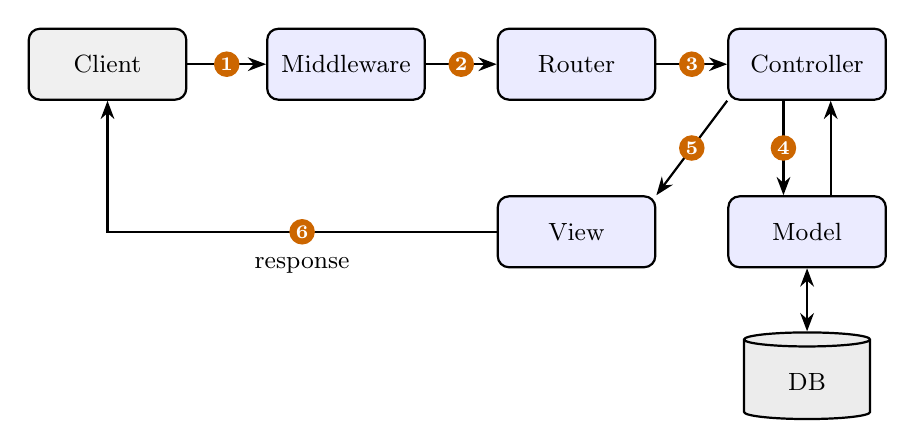
\begin{tikzpicture}[>={Stealth}, thick, node distance=9mm, every node/.style={font=\small},
    stage/.style={draw, rounded corners, fill=blue!8, minimum width=20mm, minimum height=9mm, align=center},
    num/.style={circle, fill=orange!80!black, text=white, inner sep=1pt, font=\scriptsize\bfseries}]
  \node[stage, fill=gray!12] (client) {Client};
  \node[stage, right=10mm of client] (mw) {Middleware};
  \node[stage, right=of mw] (router) {Router};
  \node[stage, right=of router] (ctrl) {Controller};
  \node[stage, below=12mm of ctrl] (model) {Model};
  \node[stage, below=12mm of router] (view) {View};
  \node[draw, cylinder, shape border rotate=90, aspect=0.25, fill=gray!15, minimum width=16mm, minimum height=11mm, below=8mm of model] (db) {DB};
  \draw[->] (client) -- node[num] {1} (mw);
  \draw[->] (mw) -- node[num] {2} (router);
  \draw[->] (router) -- node[num] {3} (ctrl);
  \draw[->] ([xshift=-3mm]ctrl.south) -- node[num] {4} ([xshift=-3mm]model.north);
  \draw[->] ([xshift=3mm]model.north) -- ([xshift=3mm]ctrl.south);
  \draw[<->] (model) -- (db);
  \draw[->] (ctrl.south west) -- node[num] {5} (view.north east);
  \draw[->] (view) -| node[pos=0.25, num] {6} node[pos=0.25, below=2mm] {response} (client);
\end{tikzpicture}
